\documentclass{article}
\usepackage{graphicx}
\usepackage{amsmath}
\usepackage{float}

\begin{document}

\section*{Algorithm Description}

\paragraph{Step 1: Sort the Points} First, sort the set of points $P$ based on their $x$-coordinates in non-increasing order. If two points have the same $x$-coordinate, then sort them by their $y$-coordinate in non-decreasing order. This pre-processing step ensures that during the merge step, we only need to compare the $y$-coordinates to determine the Pareto-optimal points, as the $x$-coordinates are already sorted.

\paragraph{Step 2: Divide and Conquer} We then employ a divide-and-conquer strategy, similar to the merge sort algorithm. Divide the sorted list of points into two halves and recursively compute the Pareto-optimal points for each half. Then, merge the two halves to construct the Pareto-optimal points for the entire set. 

During the merge step, we use two pointers to traverse both halves. Compare the points from both halves based on their $x$-coordinates (and $y$-coordinates if the $x$-coordinates are equal) and append the point with the higher $y$-coordinate to the result list if it is greater than the current maximum $y$-coordinate. This ensures that only the Pareto-optimal points are included in the merged result.

\paragraph{Step 3: Additional Points} After comparing and merging points from both halves, iterate through the remaining points in both halves, if any, and append them to the result list if their $y$-coordinate is greater than the current maximum $y$-coordinate.

\subsection*{Runtime Analysis}
The algorithm's time complexity remains $O(n \log n)$. The sorting of points takes $O(n \log n)$ time. The divide-and-conquer step also takes $O(n \log n)$ time, as we are repeatedly dividing the problem into smaller subproblems and solving each in linear time, then merging the solutions in linear time (The recurrence relation for the algorithm is given by $T(n) = 2T\left(\frac{n}{2}\right) + O(n)$, this fits the pattern of the Master Theorem, and we find that the solution is 
$T(n) = O(n \log n)$.). The use of pointers for the merge step ensures that it operates in linear time, contributing to the overall efficient performance of the algorithm.


\section*{Numerical Results}

{
\footnotesize
\begin{tabular}{|c|c|c|}
\hline
\( n \) & Normalized Experimental Time & Normalized Theoretical Time\\
\hline
10 & 0.0000244 & 0.0000035 \\
50 & 0.0001011 & 0.0000298 \\
100 & 0.0001842 & 0.0000702 \\
500 & 0.0009893 & 0.0004736 \\
1000 & 0.0015526 & 0.0010528 \\
5000 & 0.0057733 & 0.0064906 \\
10000 & 0.0161490 & 0.0140376 \\
50000 & 0.0741452 & 0.0824530 \\
100000 & 0.1645252 & 0.1754703 \\
500000 & 1.0000000 & 1.0000000 \\
\hline
\end{tabular}
}

\begin{figure}[H]
    \centering
    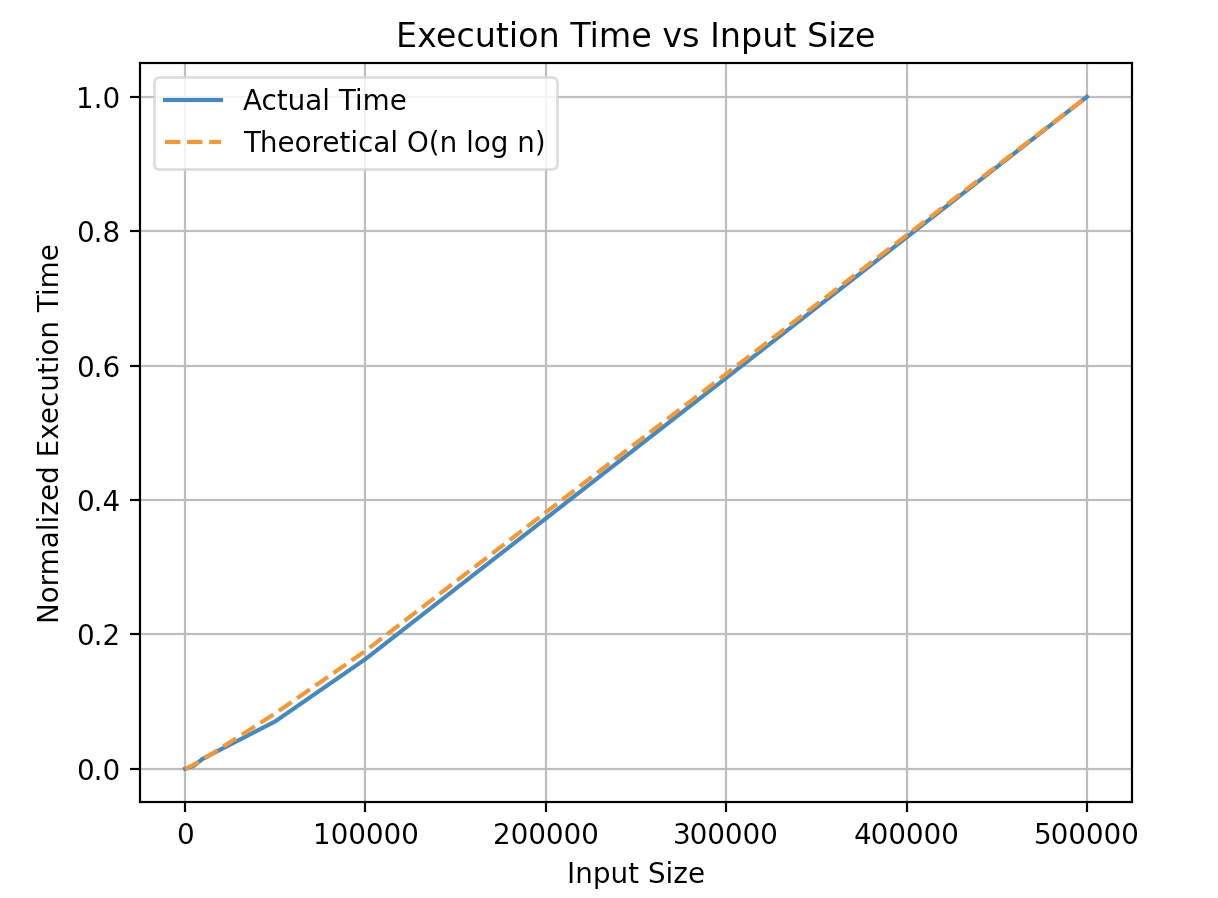
\includegraphics[width=0.8\textwidth]{image}
\end{figure}

The graph showcases an increase in execution time that aligns with an \(O(n \log n)\) time complexity, evident from the tight correspondence between the experimental and theoretical curves.

The plotted data indicates that our theoretical analysis, grounded in the divide-and-conquer strategy, is empirically valid. The slight discrepancies can be attributed to environmental and procedural variations during the execution of the algorithm, yet the overall trend aligns well with the theoretical expectation of \(O(n \log n)\) complexity.




\end{document}
